\documentclass[10pt,letterpaper,addpoints]{exam}
\usepackage[utf8]{inputenc}
\usepackage[spanish,es-noshorthands]{babel}
\usepackage{hyperref}
\usepackage{amsmath}
\usepackage{amsfonts}
\usepackage{amssymb}
\usepackage{graphicx}
\usepackage{tikz}
\usepackage{multicol}
\usepackage[width=7in,height=9.5in]{geometry}
%\printanswers
\begin{document}
\title{\begin{minipage}{.2\textwidth}
        
\includegraphics[height=1.75cm]{Images/logo-colegio.png}
       \end{minipage}
\begin{minipage}{.55\textwidth}
 \begin{center}
Prueba bimestral \\Álgebra $8^{\circ}$
\end{center}
\end{minipage}
\begin{minipage}{.2\textwidth}

\includegraphics[height=1.75cm]{Images/logo-sed.png} 
\end{minipage}
}
\author{Germ\'{a}n Avendaño Ram\'{i}rez\\Lic. Matemáticas U.D., M.Sc. U.N.}
\date{}
\maketitle
\begin{center}
\fbox{\fbox{\parbox{5.5in}{\centering
Instrucciones}}}
\end{center}
\vspace{0.1in}
\makebox[\textwidth]{Nombres: \hrulefill, curso:\underline{\hspace{48pt}}, fecha:\underline{\hspace{3cm}}}
\begin{questions}
\begin{minipage}{.65\textwidth}
\question
Una máquina corta moldes de cartón que se doblan y se pegan para construir cajas, con las medidas que se muestran en el siguiente dibujo.\\

¿Cuál de las siguientes cajas se arma con el molde del dibujo?
\end{minipage}\hfill
\begin{minipage}{.35\textwidth}
\begin{tikzpicture}
\draw (0,0) rectangle (4,1);
\draw (1,-2) rectangle (3,2);
\draw (1,-1)--(3,-1);
\draw[|-] (-.2,1)--node[below]{10cm}(-.2,.6);
\draw[|-](-.2,0)--(-.2,.4);
\draw[|-](0,-.2)--node[right]{10cm}(.1,-.2);
\draw[-|](.9,-.2)--(1,-.2);
\draw[|-](1,-2.2)--(1.5,-2.2)node[right]{20cm};
\draw[-|](2.5,-2.2)--(3,-2.2);
\draw[|-](3.2,-.1)--(3.2,-.4)node{10cm};
\draw[-|](3.2,-.6)--(3.2,-1);
\end{tikzpicture}
\end{minipage}
\begin{center}
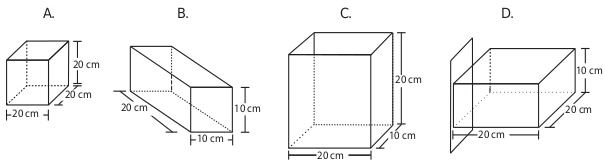
\includegraphics[scale=.75]{Images/cajas.png} 
\end{center}
\begin{minipage}{.35\textwidth}
\question
En un juego Juan lanzó tres dardos a un tablero como el siguiente:\\

El puntaje del juego se obtiene sumando los puntos asignados a la posición donde cae cada dardo.

Los tres dardos que lanzó Juan quedaron ubicados en los recuadros E5, F6 y D7.\\

¿Qué puntaje obtuvo Juan?
\end{minipage}\hfill
\begin{minipage}{.65\textwidth}
\begin{center}
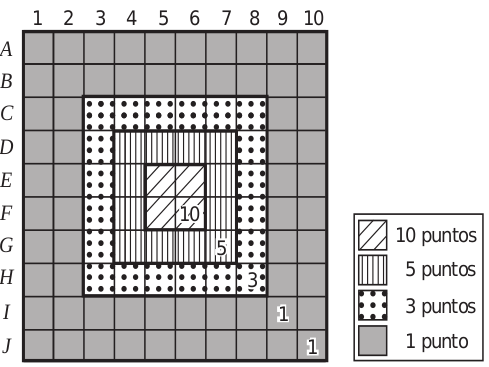
\includegraphics[scale=.55]{Images/juego_dados.png} 
\end{center}
\end{minipage}

\begin{oneparchoices}
\choice 15 puntos.
\choice 18 puntos.
\choice 20 puntos.
\CorrectChoice 25 puntos.
\end{oneparchoices}

\begin{minipage}{.5\textwidth}
\question 
La siguiente tabla muestra los nombres de los atletas de un equipo y sus respectivos pesos.

El equipo realiza algunos ejercicios en parejas. La diferencia de pesos entre los atletas que conforman una pareja no debe sobrepasar los 3 kilogramos.\\

¿Cuáles de los siguientes atletas del equipo \textbf{no} pueden realizar los ejercicios en pareja?
\end{minipage}\hfill
\begin{minipage}{.5\textwidth}
\begin{tabular}{|c|c|}
\hline 
\textbf{Nombre del atleta} & \textbf{Peso en kilogramos} \\ 
\hline 
Oscar & 60 \\ 
\hline 
Andrés & 62.5 \\ 
\hline 
Víctor & 58.6 \\ 
\hline 
Fernando & 61.3 \\ 
\hline 
César & 65.2 \\ 
\hline 
Héctor & 59.4 \\ 
\hline 
\end{tabular} 
\end{minipage}

\begin{oneparchoices}
\choice Oscar y Víctor.
\choice Fernando y Héctor.
\CorrectChoice César y Víctor.
\choice Andrés y Fernando.
\end{oneparchoices}
\question El piso de la sala de una casa tiene una superficie de 13,6 $m^{2}$. Para cubrir el piso de la sala, se van a comprar baldosas que solamente son vendidas en cajas que contienen baldosas suficientes para cubrir 2 $m^2$ de superficie.

¿Cuál es el número mínimo de cajas que se debe comprar?

\begin{oneparchoices}
\choice 6
\CorrectChoice 7
\choice 13
\choice 14
\end{oneparchoices}
\question En un almacén deportivo quieren empacar balones de 10 centímetros de radio en cajas cúbicas. Disponen de los siguientes moldes para armar las cajas
\begin{center}
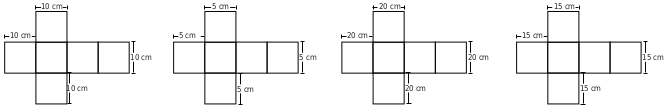
\includegraphics[scale=.75]{Images/moldes.png} 
\end{center}
¿Cuál es el molde más adecuado para construir estas cajas?

\begin{oneparchoices}
\choice El molde 1
\choice El molde 2
\CorrectChoice El molde 3
\choice El molde 4
\end{oneparchoices}
\question Cuatro atletas: Juan, Pedro, Carlos y Jorge entrenan para una competencia de atletismo, en una pista de 100 metros. Cada uno de ellos dio tres vueltas a la pista. A continuación
se relaciona el tiempo empleado por ellos en cada una de las vueltas.
\begin{center}
\begin{tabular}{|c|c|c|c|c|}
\hline 
 & \textbf{Tiempo} & \textbf{Tiempo} & \textbf{Tiempo} & \textbf{Tiempo} \\ 
\textbf{VUELTA} & \textbf{empleado por} & \textbf{empleado por} & \textbf{empleado por} & \textbf{empleado por} \\ 
 & \textbf{Juan (en segundos)} & \textbf{Pedro (en segundos)} & \textbf{Carlos (en segundos)} & \textbf{Jorge (en segundos)} \\ 
\hline 
Primera & 30 & 22 & 16 & 25 \\ 
\hline 
Segunda & 15 & 24 & 18 & 20 \\ 
\hline 
Tercera & 15 & 26 & 20 & 18 \\ 
\hline 
\end{tabular} 
\end{center}
¿Cuál de los atletas tuvo un menor tiempo por vuelta?
 
\begin{oneparchoices}
\choice Juan
\choice Pedro
\CorrectChoice Carlos
\choice Jorge
\end{oneparchoices}
\question Pablo tiene dos dados con forma de cubo, cada cara de los dados está marcada con un número distinto.

Las caras de uno de los dados están marcadas con los números 2, 4, 6, 8 ,10, 12, respectivamente.

Y las caras del otro dado, están marcadas con los números 1, 3, 5, 7, 9, 11, respectivamente.

Pablo lanza los dados, luego suma los números marcados en la cara superior de cada uno, y registra el resultado.
\\
¿Cuál de los siguientes resultados es \textbf{IMPOSIBLE} que obtenga Pablo?

\begin{oneparchoices}
\choice 11
\choice 13
\CorrectChoice 14
\choice 15
\end{oneparchoices}

\begin{minipage}{.5\textwidth}
\question Cuenta una leyenda que un rey pagó al inventor del ajedrez, un grano de maíz por el cuadrado número 1, el doble por el segundo, el doble del segundo por el tercer cuadrado y así sucesivamente. La siguiente ilustración muestra un tablero de ajedrez en el cual se han numerado algunos de sus cuadrados.\\

De acuerdo a la leyenda, ¿cuántos granos de maíz tuvo que pagar el rey, por el cuadrado número 15?
\end{minipage}\hfill
\begin{minipage}{.5\textwidth}
\begin{center}
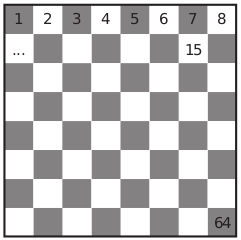
\includegraphics[scale=.8]{Images/ajedrez.png} 
\end{center}
\end{minipage}

\begin{oneparchoices}
\CorrectChoice $2^{14}$
\choice $2^{16}$
\choice $15^{2}$
\choice $2\times 15$
\end{oneparchoices}
\question En una sala de cine se organiza una rifa entre los asistentes a una de las funciones. Cada asistente marca la boleta de la entrada con sus datos y la introduce en una urna, al final de la función se extrae una boleta al azar. De los asistentes, $\frac{1}{6}$ son hombres adultos, $\frac{1}{5}$ son mujeres adultas, $\frac{1}{3}$ son niños y  $\frac{3}{10}$     son niñas. Es \textbf{menos} probable que la rifa la gane

\begin{oneparchoices}
\choice una niña
\choice un niño
\choice una mujer adulta
\CorrectChoice un hombre adulto
\end{oneparchoices}
\question Una cuadra mide 100 metros aproximadamente. Un anuncio en una tienda dice: “Gran oferta a tan sólo 1.200 metros de aquí \ldots ”. 

\end{questions}
%cuadro de puntajes
%\begin{center}
%\gradetable[h][pages]
%\end{center}
\end{document}